\chapter{Einleitung}
\begin{wrapfigure}{r}{6.5cm}
\centering
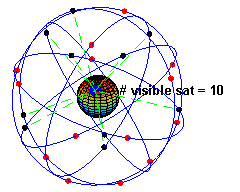
\includegraphics[scale=0.8]{Bilder/GPS.png} 
\caption{Skizze satellitengestütztes Lokalisierungssystem \cite{GPS}}
\label{GPS}
\end{wrapfigure}
Herkömmliche Navigationssysteme für den "`Outdoor"'-Bereich haben viele Handlungen des alltäglichen Lebens weitgehend erleichtert. Die Tage gehören der Vergangenheit an, in denen Fahrtstrecken über unbekannte Straßen und durch fremde Länder mit analogen Karten weit im Voraus geplant werden mussten. Die Navigation bzw. Lokalisierung basiert dabei auf einer Positionsbestimmung mithilfe von Funksignalen, die von Satelliten in der Erdumlaufbahn ausgesendet werden. Aus diesen Signalen können die Navigationssysteme ihre Position auf der Erde berechnen und schließlich dem Nutzer die Information zur Verfügung stellen. Die eigene Lokalisierung wäre nun auch für den Besucher in einem Gebäude hilfreich, damit er sich orientieren kann und beispielsweise in einem weitläufigen Kaufhaus schneller zu einem Geschäft seiner Wahl findet. Um die Vorteile einer Positionsbestimmung im "`Indoor"'-Bereich anzuwenden, können die bisherigen satellitengestützen Systeme (GPS, GLONASS, Galileo) jedoch noch nicht genutzt werden, da die massive Bauweise der Gebäude ihre Signale absorbiert bzw. reflektiert. Seit einigen Jahren arbeiten Forschungseinrichtungen und Unternehmen an einer Lösung für die Lokalisierung von Objekten im Inneren von Gebäuden. Die Forschungsprojekte verfolgen dabei viele verschiedene Ansätze und Technologien zur Erreichung dieses Ziels, wie beispielsweise die Projekte "`EVARILOS"' \cite{EVA}, "`Google Indoor Maps"' \cite{GIM} und "`Mobile Indoor Localization"' \cite{MIL} zeigen. Jedoch existiert noch keine Lösung, die sich bereits durchgesetzt hat und einen kommerziellen Nutzen erzielt.\\ \\
Eine neue und vielversprechende Technologie zur innerräumlichen Lokalisierung stellt dabei die Entwicklung von iBeacons (z. Dt. Leuchtfeuer) dar. Die Vorteile dieses Systems gegenüber bisherigen Lösungen sind zum einen die geringen Kosten sowie die hohe Flexibilität und Autonomie der einzelnen Elemente. Viele bisherigen Technologien zur Indoor-Lokalisierung, wie z.B. in den Boden eingelassene künstliche Magnetfelder \cite{Magnet}, RFID-Transponder \cite{RFID} oder funkbasierte Lösungen \cite{WLAN} sind zwar erprobt und erzielen eine hohe Lokalisierungsgenauigkeit, besitzen jedoch den Nachteil einer kostenintensiven und aufwendigen Infrastruktur, die meist auch eine bauliche Veränderung am Gebäude erfordert. Die Einfachheit der Anbringung der Beacons, die Kostenvorteile und die weitere Verbreitung des verwendeten Bluetooth-Protokolls auf mobilen Geräten sorgen dabei für ein weites Einsatzspektrum. Der größte Vorteil der iBeacons gegenüber konkurrierender Technologien stellt die variable Verwendung der Beacons beispielsweise für einfache, rudimentäre Positionsbestimmungen bis hin zur hochpräzisen Ortung dar. Je nach Einsatzszenario können die Beacons problemlos angepasst und so für ihre Bestimmung effizienter gestaltet werden.\\ \\
Nun wird für ein Lokalisierungssystem in Gebäuden ein neues Planungskonzept benötigt, das die Funkbaken optimal für ihre Aufgabe positioniert. Denn im Gegensatz zu den Satellitensystemen im Outdoor-Bereich, bewegen sich die Beacons nicht und somit können auch nicht deren Konzepte übernommen werden. Desweiteren mangelt es an Verfahren, die Gebäude mit Beacon-Systemen zweifelsfrei auf die Qualität der Lokalisierung und der räumlichen Abdeckung zu validieren. Gegenstand dieser Arbeit soll es sein, ein geeignetes Konzept für die Erstellung von Beacon-Konfigurationen zu gestalten und die Anordnung anschließend experimentell zu überprüfen. Dabei wird auf ein automatisiertes und strukturiertes Verfahren mithilfe von Robotern zurückgegriffen, um die Evaluierung weniger fehleranfällig zu designen und somit zu standardisieren.\\ \\
Aus diesen Anforderungen stellen sich drei zentrale Zielstellungen:
\begin{itemize}
\item Entwicklung eines Frameworks und einer systematischen Versuchsplanung für die Messung von Beacon-Signalen
\item Auswahl und Parameterbestimmung eines Modells für die Signalausbreitung von Beacons mit anschließender Erstellung einer Simulationsumgebung sowie einer sich daraus konkludierenden optimalen Verteilung von Beacons in einem Raum 
\item Validierung des Modells und der Simulationsergebnisse in einem Testszenario mithilfe eines Roboters  
\end{itemize}
Um die Problematik eines bisher fehlenden Planungskonzeptes darzulegen, wird zuerst der Stand der Technik von Beacons beschrieben und erläutert. Daraus schlussfolgern sich in Kapitel 3 erste Ansätze darüber wie ein mögliches Verfahren zur Beacon-Konfiguration aufgebaut sein muss. In Kapitel 4 werden für die erste Zielsetzung, der Modellierung von Beacons, alle Werkzeuge zur Messung der Beacon-Signale vorgestellt und ausgewertet. Mit den Messwerten werden anschließend die Parameter für die Signalausbreitung der Beacons in einem freien Raum bestimmt und damit die Grundlage für ein Simulationsprogramm gelegt. Da noch keine bekannten Veröffentlichungen über die Lokalisierungsgenauigkeit mittels Beacons existieren, wird zusätzlich aus den Messwerten dafür eine Qualitäts-Skala bestimmt und diese erklärt. Mithilfe der Simulation und eines Optimierungsalgorithmus werden anhand der selbstdefinierten Qualitätskriterien geeignete Beacon-Konfigurationen berechnet und diese experimentell in Kapitel 7 überprüft. Dhingehend wird im Anschluß besonders auf die Vorhersage-Genauigkeit aller getroffenen Annahmen eingegangen und die statischen Messungen mit den dynamischen verglichen. Am Ende der Arbeit werden die drei verfassten Zielstellungen mit dem Erreichten gegenüber gestellt, die Ergebnisse daraus diskutiert und anschließend wird das Konzept danach bewertet. 
 





% Bietet sich leider hier nicht an:(

%Zur Anschaulichkeit sind nachfolgend in Abbildung ... alle funkbasierte Verfahren zur Entfernungsmessung einmal vorgestellt.
%
%\begin{tikzpicture}[level 1/.style={sibling distance=40mm}, edge from parent/.style={->,draw}, >=latex]
%% root of the the initial tree, level 1
%\node[root] {HF-basierende Entfernungsmessungen}
%% The first level, as children of the initial tree
%  child {node[level 2] (c1) {Defining node and arrow styles}}
%  child {node[level 2] (c2) {Positioning the nodes}}
%  child {node[level 2] (c3) {Drawing arrows between nodes}};
%
%% The second level, relatively positioned nodes
%\begin{scope}[every node/.style={level 3}]
%\node [below of = c1, xshift=15pt] (c11) {Setting shape};
%\node [below of = c11] (c12) {Choosing color};
%\node [below of = c12] (c13) {Adding shading};
%
%\node [below of = c2, xshift=15pt] (c21) {Using a Matrix};
%\node [below of = c21] (c22) {Relatively};
%\node [below of = c22] (c23) {Absolutely};
%\node [below of = c23] (c24) {Using overlays};
%
%\node [below of = c3, xshift=15pt] (c31) {Default arrows};
%\node [below of = c31] (c32) {Arrow library};
%\node [below of = c32] (c33) {Resizing tips};
%\node [below of = c33] (c34) {Shortening};System
%\node [below of = c34] (c35) {Bending};
%\end{scope}
%
%% lines from each level 1 node to every one of its "children"
%\foreach \value in {1,2,3}
%  \draw[->] (c1.195) |- (c1\value.west);
%
%\foreach \value in {1,...,4}
%  \draw[->] (c2.195) |- (c2\value.west);
%
%\foreach \value in {1,...,5}
%  \draw[->] (c3.195) |- (c3\value.west);
%\end{tikzpicture} 
%
%\cite{IndLoc} und \cite{DisLok}
